\documentclass{article}
\usepackage[top=1.0in,bottom=1.0in,left=1.0in,right=1.0in]{geometry}
\usepackage{amsmath,amssymb,amsthm,amsfonts}
\usepackage[utf8]{inputenc}
\usepackage{hyperref}
\usepackage{graphics,graphicx}

\title{Triptych-2: efficient proofs for confidential transactions}
\author{Sarang Noether \\ Monero Research Lab \\ \texttt{sarang.noether@protonmail.com}}
\date{\today}

\newcommand{\G}{\mathbb{G}}
\newcommand{\F}{\mathbb{F}}
\newcommand{\N}{\mathbb{N}}
\newcommand{\hs}{\mathsf{H}}
\newcommand{\hp}{\mathcal{H}}
\newcommand{\com}{\operatorname{Com}}
\newcommand{\A}{\mathcal{A}}

\newcommand{\sumi}{\sum_{i=0}^{n-1}}
\newcommand{\sumj}{\sum_{j=0}^{m-1}}
\newcommand{\sumk}{\sum_{k=0}^{N-1}}
\newcommand{\sumu}{\sum_{u=0}^{w-1}}

\newtheorem{theorem}{Theorem}
\theoremstyle{definition}
\newtheorem{definition}{Definition}


\begin{document}

\maketitle


\begin{abstract}
Confidential transactions are used in distributed digital assets to demonstrate the balance of values hidden in commitments, while retaining signer ambiguity.
Previous work describes a signer-ambiguous proof of knowledge of the opening of commitments to zero at the same index across multiple public commitment sets and the evaluation of a verifiable random function used as a linking tag, and uses this to build a linkable ring signature called Triptych that can be used as a building block for a confidential transaction model.
In this work, we extend Triptych to build Triptych-2, a proving system that proves knowledge of openings of multiple commitments to zero within a single set, correct construction of a verifiable random function evaluated at each opening, and value balance across a separate list of commitments within a single proof.
While soundness depends on a novel dual discrete-logarithm hardness assumption, we use data from the Monero blockchain to show that Triptych-2 can be used in a confidential transaction model to provide faster total batch verification time than other state-of-the-art constructions without a trusted setup.
\end{abstract}


\section{Introduction}
Distributed digital assets, starting with Bitcoin, rely on digital signatures to authorize transactions and transfer the spend authority of funds.
While early protocols based on the model established by Bitcoin have the advantage of simplicity, they lack desirable properties relating to privacy and indistinguishability.
In particular, the address and signature graph formed by the blockchain in such assets is trivially traceable, and the amounts a signature authorizes in a transaction are visible.

To protect users of distributed assets and permit better indistinguishability of transactions for fungibility, several methods have been proposed and deployed toward confidential transactions.
The CryptoNote protocol, an early proposal for obscuring transaction graphs, relies on linkable ring signatures on transaction outputs with denominated amounts \cite{cryptonote}; a transaction includes a separate signature for each such amount, yielding poor scaling.
A later advancement to the RingCT protocol \cite{ringct} used Pedersen commitments to amounts associated with transaction outputs and extended a ring signature construction by Liu \text{et al.} \cite{liu} to support parallel signatures in a matrix arrangement, removing the need for denominated transaction outputs altogether.
However, both of these constructions use linkable ring signatures that scale linearly in size with the size of the anonymity set used in each signature.

More recent methods of maintaining transaction privacy use accumulators to represent a given state of transaction outputs.
Zerocoin \cite{zerocoin} relied on RSA accumulators and associated proofs to assert the validity of transactions, but amounts were fixed, the protocol used very large and inefficient proofs, transactions were limited to a simple burn-mint operation on a transparent chain, and the use of RSA groups required a trusted setup process.
Later work produced Zerocash \cite{zerocash}, which replaced RSA accumulators and related proofs with succinct proofs relating to Merkle tree accumulators, enabling arbitrary amounts and direct anonymous transfers.
However, like Zerocoin, Zerocash used a proving system requiring a trusted setup process; this was eventually used as the basis for the Zcash protocols.

Until recently, transaction protocols desiring robust signer ambiguity and flexible direct anonymous transfers of arbitrary amounts faced a tradeoff between a trust-free construction and efficiency in proof sizes and verification complexity.
Recent work in this area generally relies on one of two novel proving systems to build transactions that scale in size logarithmically with the size of the prover-specified anonymity set, while requiring no trusted setup.
A one-of-many commitment-to-zero proving system of Groth and Kohlweiss \cite{groth} was used to build simple ring signatures and Zerocoin-style transactions, and was later extended to support accountable ring signatures more efficiently by Bootle \cite{bootle}.
This proving system forms the basis of Lelantus \cite{lelantus}, which extends the Zerocoin-style transaction model of \cite{groth} by using multiple-base Pedersen commitments to incorporate amounts alongside serial numbers; a modification to the proofs shows balance, and multiple proofs are needed for typical transactions.
However, Lelantus transactions allow a transaction sender to later identify when the recipient spends their funds; a mitigation to this solves the tracing problem, but at the cost of eliminating a useful one-time addressing construction that ensures recipient anonymity.
The same proving system in \cite{groth} is used in Triptych \cite{triptych}, a multi-dimensional linkable ring signature construction that can be used to build confidential transactions similarly to \cite{ringct}; Triptych notably supports one-time addressing and arbitrary amounts, while still requiring the use of multiple proofs for transactions spending multiple transaction outputs.
Interestingly, recent independent work extends \cite{groth} to support proofs on multiple commitments in a single list (as we also introduce below), with a particular application to Zether \cite{zether}; however, this uses a different approach than we take here, and seems to result in larger proofs.

The Bulletproofs \cite{bulletproofs} proving system uses an inner-product compression method to build range and circuit satisfiability proofs with logarithmic size scaling.
Besides an increasingly widespread deployment for commitment range proofs, the underlying structure of Bulletproofs is used to construct more specialized proving systems for confidential transactions.
Omniring \cite{omniring} uses this method to build transactions that demonstrate spend authorization for multiple signer-ambiguous transaction inputs within a single proof, while directly integrating range proving.
The result is very small proofs; however, verification is slower than other approaches, and requirements for unique group generators mean such proofs cannot be verified in efficient batches.
RingCT 3.0 \cite{rct3} also uses a Bulletproof-style construction.
In an early version, transactions required separate proofs for multiple inputs; while an update incorporates a single proof for all inputs to a transaction, it also requires that the number of inputs be padded to a power of two, which can yield poor verification complexity.


\subsection{Our contribution}
We extend the proving system in Triptych \cite{triptych} in two significant ways, which we call Triptych-2.
First, we enable the prover to show knowledge of multiple signing keys in a single proof simultaneously using one set of combined proof elements; unlike \cite{rct3}, our modification admits any number of transaction inputs without limitations.
We retain the verifiable random function evaluation that produces linking tags, which are required for the detection of repeat signing with the same commitment opening across proofs.
Second, we show Pedersen commitment value balance directly within the same proof; in particular, we show that a particular combination of input and output commitments sums to a commitment to zero.
We note that the soundness of the resulting proving system depends on a novel dual discrete-logarithm hardness assumption that we are not able to reduce to a standard hardness assumption; while we consider this novel assumption reasonable, it is untested.

Taken together, these changes have application to a transaction protocol for efficient use in blockchain confidential transactions that does not require any trusted setup process.
A transaction can sign for multiple signer-ambiguous inputs and prove that the transaction balances using a single proof, a major improvement to currently-deployed constructions that require multiple proofs and separate auxiliary Pedersen amount commitments.
Further, we use actual blockchain data from the Monero digital asset project to directly compare the overall size and verification time of Triptych-2 to that of Triptych and two separate RingCT 3.0 constructions.
We find that Triptych-2 provides superior verification performance compared to other trust-free confidential transaction constructions, with competitive size scaling.


\section{Preliminaries}
\subsection{Public parameters}
Let $\G$ be a cyclic group in which the discrete logarithm problem is hard, and let $\F$ be its scalar field.
Let $\hs: \{0,1\}^* \to \F$ and $\hp: \{0,1\}^* \to \G$ be cryptographic hash functions.
Let $N = n^m$ be a positive integer, where $m > 1$ (for our construction, we will use $n = 2$.
Assume that $G$, $H$, $U$, and any point of the form $G_i$ or $H_i$ (possibly with multiple indices) are uniformly random generators of $\G$ whose discrete logarithm relationship to each other is unknown.
Note that all such generators may be produced using public randomness; for example, the use of a suitable hash function with domain separation may be appropriate.
All such public parameters are assumed to comprise a global reference string known to all players; in particular, we generally exclude explicit reference to public parameters from algorithm definitions and Fiat-Shamir transcript hashes for readability.


\subsection{Tensor commitment}
Let $\com$ be an additively homomorphic commitment scheme that is perfectly hiding and (at least) computationally binding.
In this work, we assume use of a simple extension to the Pedersen commitment scheme: for $x,r \in \F$, define $\com(x,r) \equiv rG + xH$ to be the commitment of the value $x$ with randomness $r$.

For a three-dimensional tensor $f \equiv (f_{i,j,k}) \subset \F$ and blinding factor $r \in \F$, define the Pedersen tensor commitment
$$\com(f,r) \equiv rG + \sum_{i,j,k} f_{i,j,k} G_{i,j,k}$$
using fixed independent generators as described above.

Operations on tensors are assumed to be performed componentwise; for example, if $f \equiv (f_{i,j,k})$ and $g \equiv (g_{i,j,k})$ are such tensors over $\F$, then $f + g \equiv (f_{i,j,k} + g_{i,j,k})$, and so forth.


\subsection{Other notation}
For integers or field elements $i,j$, the Kronecker delta function $\delta(i,j)$ evaluates to $1$ if $i=j$ and $0$ otherwise, where the output is taken to be in the appropriate set.

We sometimes use index subscript notation of the form $i_j$ to indicate the $j$ digit of $i$, where such a decomposition of $i$ is taken base $n$ with padded length $m$:
$$\sum_{j=0}^{m-1} i_j n^j = i$$
This notation will be specified explicitly where confusion may occur.


\subsection{Sigma protocols}
For a given relation $\mathcal{R}$, a sigma protocol for $\mathcal{R}$ is an interactive challenge-response protocol between a prover and verifier, where the prover wishes to convince the verifier it knows a witness corresponding to a statement in $\mathcal{R}$.

A sigma protocol is complete, sound, and zero-knowledge.
These definitions are well known and found, for example, in \cite{groth}.
Essentially, these properties are:
\begin{itemize}
\item \textit{Perfectly complete}: For a witness to a statement in $\mathcal{R}$, an honest prover always convinces an honest verifier of the validity.
\item \textit{Special sound}: Given a statement in $\mathcal{R}$, if the prover can produce valid proof transcripts in response to multiple verifier challenges, then it is possible to extract a witness for the statement from the transcripts.
\item \textit{Special honest-verifier zero knowledge}: Given a statement and known verifier challenge, it is possible to produce a simulated transcript without knowledge of a corresponding valid witness.
\end{itemize}
Sigma protocols can be made non-interactive by replacing random verifier challenges with hash-based transcript challenges under the random oracle model; this approach is called the Fiat-Shamir heuristic \cite{fiat}.


\subsection{Hardness assumption}
We now define a novel cryptographic hardness assumption that is used later to show the soundness of our construction.

\begin{definition}[Dual-target discrete logarithm problem]
\label{def:dual}
Let $\G$ be a group in which the discrete logarithm problem is hard, and let $\F$ be its scalar field.
Let $n > 0$.
Consider the following game between a challenger and a probabilistic polynomial-time player $\A$:
\begin{itemize}
\item The challenger chooses $G,H \in \G$ uniformly at random and sends both to $\A$.
\item $\A$ chooses and returns sets $\{G_i\}_{i=0}^{n-1},\{H_i\}_{i=0}^{n-1} \subset \G$ to the challenger.
\item The challenger chooses a set $\{\mu_i\}_{i=0}^{n-1} \subset \F$ uniformly at random and sends it to $\A$.
\item $\A$ chooses and returns a set $\{x_i\}_{i=0}^{n-1} \subset \F$ to the challenger.
\end{itemize}
We say that $\A$ wins the $(n,\epsilon,t)$-dual-target discrete logarithm game if, in time less than $t$ and with probability at least $\epsilon$, the following are true:
\begin{itemize}
\item $\sumi \mu_i \left( G_i - x_iG \right) = 0$
\item $\sumi \mu_i \left( H - x_iH_i \right) = 0$
\item There exists an index $0 \leq i < n$ such that either $x_iG \neq G_i$ or $x_iH_i \neq H$.
\end{itemize}
\end{definition}


\section{Proving system}
We now present a sigma protocol for the following relation:
\begin{multline*}
\mathcal{R} \equiv \Bigg\{ \{M_i\}_{i=0}^{N-1},\{P_i\}_{i=0}^{N-1},\{J^{(u)}\}_{u=0}^{w-1},\{Q_j\}_{j=0}^{T-1} \subset \G \: ; \: \left( \{l^{(u)}\}_{u=0}^{w-1}, \{r^{(u)}\}_{u=0}^{w-1}, y \right) : \\
M_{l^{(u)}} = r^{(u)}G \; \forall \: u \in [0,w) \text{ and } r^{(u)}J^{(u)} = U \; \forall \: u \in [0,w) \text{ and } \sum_{u=0}^{w-1} P_{l^{(u)}} - \sum_{j=0}^{T-1} Q_j = yG \Bigg\}
\end{multline*}
This captures the necessary elements for transaction authorization, which we describe later; knowledge of signing keys $\{r^{(u)}\}$ will show that the prover has signing authority for inputs to a transaction, and knowledge of the secret key $y$ to an amount commitment difference will show that the transaction amounts balance.
Finally, comparison of the verifiable random function used to produce $\{J^{(u)}\}$ will be used to prevent attempts to sign for the same secret key without revealing the corresponding public key, which is important for signer ambiguity and double-spend protection within or between proofs.

Figures \ref{fig:sigma} and \ref{fig:sigma2} describe the prover and verifier interaction.
Next, we prove that the prover and verifer routines constitute a sigma protocol that is perfectly correct, special sound, and special honest-verifier zero knowledge.

\begin{figure}[htbp]
\centering
\fbox{\begin{minipage}{0.95\textwidth}
$\underline{\mathcal{P}:}$
\begin{itemize}
\item Select random $r_A \in \F$ and $\left\{a_{j,i}^{(u)}\right\}_{i=1,j,u=0}^{n-1,m-1,w-1} \subset \F$.
Set $$\{a_{j,0}^{(u)}\}_{j,u=0}^{m-1,w-1} \equiv -\sum_{i=1}^{n-1} a_{j,0}^{(u)}$$ and define $A \equiv \com(a,r_A)$.
\item Define $\left\{\sigma_{j,i}^{(u)}\right\}_{i,j,u=0}^{n-1,m-1,w-1} \subset \F$ such that $\sigma_{j,i}^{(u)} \equiv \delta\left(l_j^{(u)},i\right)$ (using our decomposition notation), and choose random $r_B \in \F$.
Define $B \equiv \com(\sigma,r_B)$.
\item Select random $r_C \in \F$, and define $C \equiv \com(a(1-2\sigma), r_C)$.
\item Select random $r_D \in \F$, and define $D \equiv \com(-a^2, r_D)$.
\item For $0 \leq u < w$, define coefficients $\left\{p_{k,j}^{(u)}\right\}_{k,j=0}^{N-1,m-1}$ such that $$p_k^{(u)}(x) \equiv \prod_{j=0}^{m-1} \left( \sigma_{j,k}^{(u)}x + a_{j,k}^{(u)} \right) = \delta\left(l^{(u)},k\right)x^m + \sumj p_{k,j}^{(u)}x^j$$ (using our decomposition notation).
Then define $p_{k,j} \equiv \sumu p_{k,j}^{(u)}$ and $p_k(x) \equiv \sumu p_k^{(u)}(x)$ accordingly.
\item Select random $\left\{\rho_j\right\}_{j,u=0}^{m-1,w-1}, \left\{\overline{\rho}_j^{(u)}\right\}_{j,u=0}^{m-1,w-1} \subset \F$.
\item Define aggregation coefficients $\{\mu_k\}_{k=0}^{N-1}$ using a $k$-indexed $\hs$ operation, containing all Fiat-Shamir transcript public parameters and proof elements.
\item Define $\{X_j\}_{j=0}^{m-1} \subset \G$ such that: $$X_j \equiv \sumk p_{k,j}\mu_kM_k + \sumu \rho_j^{(u)}G$$
\item Define $\{Y_j\}_{j=0}^{m-1} \subset \G$ such that: $$Y_j \equiv U \sumk p_{k,j}\mu_k + \sumu \rho_j^{(u)}J^{(u)}$$
\item Define $\{Z_j\}_{j=0}^{m-1} \subset \G$ such that: $$Z_j \equiv \sumk p_{k,j}P_k + \sumu \overline{\rho}_j^{(u)}G$$
\end{itemize}

$\underline{\mathcal{P} \to \mathcal{V}:}$ \\
$A,B,C,D,\{X_j\},\{Y_j\},\{Z_j\}$
\end{minipage}}
\caption{Sigma protocol for $\mathcal{R}$}
\label{fig:sigma}
\end{figure}

\begin{figure}[htbp]
\centering
\fbox{\begin{minipage}{0.95\textwidth}
$\underline{\mathcal{V} \to \mathcal{P}:}$ \\
$\xi \in \{0,1\}^*$ \\

$\underline{\mathcal{P}(\xi):}$
\begin{itemize}
\item Define $\left\{f_{j,i}^{(u)}\right\}_{i=1,j,u=0}^{n-1,m-1,w-1}$ such that $f_{j,i}^{(u)} \equiv \sigma_{j,i}^{(u)}\xi + a_{j,i}^{(u)}$.
\item Define $z_A \equiv r_A + \xi r_B$ and $z_C \equiv \xi r_C + r_D$.
\item Define $\left\{z_R^{(u)}\right\}_{u=0}^{w-1} \subset \F$ such that: $$z_R^{(u)} \equiv \mu_{l^{(u)}}r^{(u)}\xi^m - \sumj \rho_j^{(u)}\xi^j$$
\item Define: $$z_S \equiv \xi^m \left( \sumu s^{(u)} - \sum_{j=0}^{T-1} t_j \right) - \sumj \left( \xi^j \sumu \overline{\rho}_j^{(u)} \right)$$
\end{itemize}

$\underline{\mathcal{P} \to \mathcal{V}:}$ \\
$\{f_{j,i}^{(u)}\}_{j=0,i=1,u=0}^{m-1,n-1,w-1},z_A,z_C,\{z_R^{(u)}\},z_S$ \\

$\underline{\mathcal{V}:}$
\begin{itemize}
\item For $0 \leq u < w$ and $0 \leq j < m$, set: $$f_{j,0}^{(u)} \equiv \xi - \sum_{i=1}^{n-1} f_{j,i}^{(u)}$$
\item Accept if and only if:
\begin{eqnarray}
A + \xi B &=& \com(f,z_A) \label{eqn:ab} \\
\xi C + D &=& \com(f(\xi-f),z_C) \label{eqn:cd} \\
\sumk \mu_kM_k \left[ \sumu \left( \prod_{j=0}^{m-1} f_{j,k_j}^{(u)} \right) \right] - \sumj \xi^jX_j - \sumu z_R^{(u)}G &=& 0 \label{eqn:x} \\
U \sumk \mu_k \left[ \sumu \left( \prod_{j=0}^{m-1} f_{j,k_j}^{(u)} \right) \right] - \sumj \xi^jY_j - \sumu z_R^{(u)}J^{(u)} &=& 0 \label{eqn:y} \\
\sumk P_k \left[ \sumu \left( \prod_{j=0}^{m-1} f_{j,k_j}^{(u)} \right) \right] - \sumj \xi^jZ_j - \xi^m\sum_{j=0}^{T-1} Q_j - z_SG &=& 0 \label{eqn:z}
\end{eqnarray}
\end{itemize}
\end{minipage}}
\caption{Sigma protocol for $\mathcal{R}$ (continued)}
\label{fig:sigma2}
\end{figure}


\section{Security}
\begin{theorem}
The sigma protocol in Figures \ref{fig:sigma} and \ref{fig:sigma2} reflects the relation $\mathcal{R}$ and is perfectly correct, $(m+1)$-special sound, and special honest-verifier zero knowledge.
\end{theorem}

\begin{proof}
The proof proceeds similarly to that of \cite{triptych}, which in turn follows the methods in \cite{groth,bootle}.

To show the protocol is perfectly complete, suppose a verifier receives an honest proof.
We wish to show that all verifier equations hold.
Equation \ref{eqn:ab} holds from the identity $$\sumi \sigma_{j,i}^{(u)} = 1$$ for all $0 \leq j < m$ and $0 \leq u > w$.
Similarly, Equation \ref{eqn:cd} holds from the identity $$(\sigma_{j,i}^{(u)})^2 = \sigma_{j,i}^{(u)}$$ for all $0 \leq i < n$ and $0 \leq j < m$ and $0 \leq u < w$.

Next, we show that Equation \ref{eqn:x} holds:
\begin{eqnarray*}
&& \sumk \mu_kM_k \left[ \sumu \left( \prod_{j=0}^{m-1} f^{(u)}_{j,k_j} \right) \right] - \sumj x^jX_j - \sumu z^{(u)}_RG \\
&=& \sumk \mu_kM_k p_k(x) - \sumj x^j \left( \sumk p_{k,j}\mu_kM_k + \sumu \rho^{(u)}_jG \right) - \sumu z^{(u)}_RG \\
&=& \sumk \mu_kM_k \left( p_k(x) - \sumj x^j p_{k,j} \right) - \sumj x^j \sumu \rho^{(u)}_jG - \sumu z^{(u)}_RG \\
&=& \sumk \mu_kM_k \left[ x^m \sumu \delta\left( l^{(u)},k \right) \right] - \sumj x^j \sumu \rho^{(u)}_jG - \sumu\left[ \mu_{l^{(u)}}r^{(u)}x^m - \sumj \rho^{(u)}_jx^j \right]G \\
&=& x^m\sumu \mu_{l^{(u)}}r^{(u)}G - \sumj x^j \sumu \rho^{(u)}_jG - x^m\sumu \mu_{l^{(u)}}r^{(u)}G + \sumj x^j \sumu \rho^{(u)}_jG \\
&=& 0
\end{eqnarray*}

Equation \ref{eqn:y} holds with similar algebra:
\begin{eqnarray*}
&& \sumk \mu_kU \left[ \sumu \left( \prod_{j=0}^{m-1} f^{(u)}_{j,k_j} \right) \right] - \sumj x^jY_j - \sumu z^{(u)}_RJ^{(u)} \\
&=& \sumk \mu_kU p_k(x) - \sumj x^j \left( \sumk p_{k,j}\mu_kU + \sumu \rho^{(u)}_jJ^{(u)} \right) - \sumu z^{(u)}_RJ^{(u)} \\
&=& \sumk \mu_kU \left( p_k(x) - \sumj x^j p_{k,j} \right) - \sumj x^j \sumu \rho^{(u)}_jJ^{(u)} - \sumu z^{(u)}_RJ^{(u)} \\
&=& \sumk \mu_kU \left[ x^m \sumu \delta\left( l^{(u)},k \right) \right] - \sumj x^j \sumu \rho^{(u)}_j(r^{(u)})^{-1}U - \sumu\left[ \mu_{l^{(u)}}r^{(u)}x^m - \sumj \rho^{(u)}_jx^j \right](r^{(u)})^{-1}U \\
&=& x^m\sumu \mu_{l^{(u)}}U - \sumj x^j \sumu \rho^{(u)}_j(r^{(u)})^{-1}U - x^m\sumu \mu_{l^{(u)}}U + \sumj x^j \sumu \rho^{(u)}_j(r^{(u)})^{-1}U \\
&=& 0
\end{eqnarray*}

Finally, we show that Equation \ref{eqn:z} holds:
\begin{eqnarray*}
&& \sumk P_k \left[ \sumu \left( \prod_{j=0}^{m-1} f^{(u)}_{j,k_j} \right) \right] - \sumj x^jZ_j - x^m\sum_{j=0}^{T-1} Q_j - z_SG \\
&=& \sumk P_k p_k(x) - \sumj x^j \left( \sumk p_{k,j}P_k + \sumu \overline{\rho}^{(u)}_jG \right) - x^m\sum_{j=0}^{T-1} Q_j - z_SG \\
&=& \sumk P_k \left( p_k(x) - \sumj x^j p_{k,j} \right) - \sumj x^j \sumu \overline{\rho}^{(u)}_jG - x^m\sum_{j=0}^{T-1} Q_j - z_SG \\
&=& x^m\sumu (s^{(u)}G + a_uH) - \sumj x^j \sumu \overline{\rho}^{(u)}_jG - x^m\sum_{j=0}^{T-1} (t_jG + b_jH) - x^m\left( \sumu s^{(u)} - \sum_{j=0}^{T-1} t_j \right)G + \\
&& \sumj x^j \sumu \overline{\rho}^{(u)}_jG \\
&=& \left( \sumu a_u - \sum_{j=0}^{T-1} b_j \right)H \\
&=& 0
\end{eqnarray*}
Hence, the protocol is perfectly complete.

Next, we show that the sigma protocol is special honest-verifier zero knowledge.
To do so, we construct a simulator that, when given a random verifier challenge $\xi$, can construct a proof transcript with identical distribution to a valid proof.

Observe first that the simulator presented in the proof of Lemma 1 in \cite{bootle} translates nearly identically to our setting, since we can flatten tensor commitments to a matrix structure with the required sum property.
The simulator first chooses $B \in \G$ uniformly at random; then, the cited lemma assures a valid simulation of the proof elements  $A,C,D,z_A,z_C,\{f^{(u)}_{j,i \neq 0}\}$, and from this we may compute $\{f^{(u)}_{j,0}\}$.
In a valid proof, $B$ is also uniformly distributed.

The proof elements $\{X_j\}_{j=1}^{m-1},\{Y_j\}_{j=1}^{m-1}, \{Z_j\}_{j=1}^{m-1}$ are independent and uniformly distributed in a valid proof since the elements of $\{\rho_j\},\{\overline{\rho}_j\}$ are uniformly distributed and the discrete logarithm problem in $\G$ is hard; hence, the simulator chooses them uniformly at random.
Since the verification checks require that $X_0,Y_0,Z_0$ be uniquely determined by the other elements in the respective sets, they are selected by the simulator in this manner.

Finally, the elements $\{z^{(u)}_R\}_{u=0}^{w-1}$ and $z_S$ are independent and uniformly distributed in valid proofs given a random verifier challenge $\xi$, so the simulator may choose them uniformly at random.
Hence the protocol is special honest verifier zero-knowledge.

We claim that the protocol is $(m+1)$-special sound, where $m > 1$.
To show this, we construct an extractor that, when given $m+1$ valid responses to $m+1$ distinct verifier challenges for the same initial statement, produces a valid witness for the statement.
In particular, we produce a modified witness for the following relation that is based on the information presented in the prover algorithm, where we define aggregation coefficients $\mu_k$ as before:
\begin{multline*}
\mathcal{R}' \equiv \Bigg\{ \{M_k\}_{k=0}^{N-1},\{P_k\}_{k=0}^{N-1},\{J^{(u)}\}_{u=0}^{w-1},\{Q_j\}_{j=0}^{T-1} \subset \G \: ; \: \left( \{l^{(u)}\}_{u=0}^{w-1}, \{r^{(u)}\}_{u=0}^{w-1}, y \right) : \\
\sumu \mu_{l^{(u)}} M_{l^{(u)}} = \sumu \mu_{l^{(u)}} r^{(u)}G \text{ and } \sumu \mu_{l^{(u)}} r^{(u)}J^{(u)} = \sumu \mu_{l^{(u)}} U \text{ and } \sum_{u=0}^{w-1} P_{l^{(u)}} - \sum_{j=0}^{T-1} Q_j = yG \Bigg\}
\end{multline*}
Observe that if we assume that the dual-target discrete logarithm problem is hard in $\G$, extraction of a witness for $\mathcal{R}'$ implies knowledge of a corresponding witness for $\mathcal{R}$; this in turn provides the desired soundness.

Suppose that for a given statement, we have a set of $(m+1)$ distinct verifier challenges $\{\xi_e\}_{e=0}^m$ corresponding to distinct valid responses of this form:
$$\left\{ \{{}_ef^{(u)}_{j,i}\}, \{{}_ez^{(u)}_R\}, {}_ez_S \right\}_{e=0}^m$$
From the $3$-special soundness in \cite{bootle} and $m > 1$ we have valid extractions $\{\sigma^{(u)}_{j,i}\}_{u=0}^{w-1}$ and $\{a^{(u)}_{j,i}\}_{u=0}^{w-1}$, and the Pedersen binding property ensures that (with high probability) we have:
$${}_ef^{(u)}_{j,i} = \sigma^{(u)}_{j,i}\xi_e + a^{(u)}_{j,i} \; \forall \: e \in [0,m]$$
Using the extracted values, compute the polynomial
$$p_k(x) \equiv \sum_{u=0}^{w-1}\left[ \prod_{j=0}^{m-1} \left( \sigma^{(u)}_{j,k}x + a^{(u)}_{j,k} \right) \right]$$
for all $k \in [0,N)$.
Extraction of $\{\sigma^{(u)}_{j,i}\}_{u=0}^{w-1}$ immediately yields the signing index set $\{l^{(u)}\}_{u=0}^{w-1}$.

We have seen that $p_k$ is of degree $m$ only when $k \in \{l^{(u)}\}_{u=0}^{w-1}$.
Hence there exist sets of coefficients $\{\overline{X}_j,\overline{Y}_j,\overline{Z}_j\}_{j=0}^{m-1}$, computed uniquely from the statement and extracted values, such that Equations \ref{eqn:x}, \ref{eqn:y}, and \ref{eqn:z} are of the following form:
\begin{eqnarray*}
\xi^m \sumu \mu_{l^{(u)}}M_{l^{(u)}} + \sumj \xi^j\overline{X}_j &=& \left( \sumu z^{(u)}_R \right)G \\
\xi^m \sumu \mu_{l^{(u)}}U + \sumj \xi^j\overline{Y}_j &=& \sumu z^{(u)}_RJ^{(u)} \\
\xi^m \sumu P_{l^{(u)}} + \sumj \xi^j\overline{Z}_j - \xi^m \sum_{j=0}^{T-1} Q_j &=& z_SG
\end{eqnarray*}

Construct a Vandermonde matrix $V$ where the $e$ row is the vector $(1,\xi_e,\ldots,\xi^m_e)$.
Since all $\xi_e$ are distinct, the rows of $V$ span $\F^{m+1}$; hence there exist weights $\{\theta_e\}_{e=0}^m$ such that the resulting linear combination of rows produces the vector $(0,\ldots,0,1)$.
That is, $\sum_{e=0}^m \theta_e\xi_e^j = \delta(j,m)$.

For each of the previous three equations, we can therefore build a linear combination over $e$. For the first:
$$\sumu \mu_{l^{(u)}} M_{l^{(u)}} = \sum_{e=0}^m \theta_e\xi_e^m \left( \sumu \mu_{l^{(u)}} M_{l^{(u)}} \right) + \sum_{e=0}^m \theta_e \left( \sumj \xi_e^j \overline{X}_j \right) = \sumu \left( \sum_{e=0}^m \theta_e {}_ez^{(u)}_R \right) G$$
We therefore can define extractions for each $r^{(u)}$:
$$r^{(u)} \equiv \frac{1}{\mu_{l^{(u)}}} \sum_{e=0}^m \theta_e {}_ez^{(u)}_R$$
Observe that the same witnesses appear in the second:
$$\sumu \mu_{l^{(u)}} U = \sum_{e=0}^m \theta_e\xi_e^m \left( \sumu \mu_{l^{(u)}} U \right) + \sum_{e=0}^m \theta_e \left( \sumj \xi_e^j \overline{Y}_j \right) = \sumu \left( \sum_{e=0}^m \theta_e {}_ez^{(u)}_R \right) J^{(u)}$$
This means the requirements on each $r^{(u)}$ are satisfied. The third equation proceeds similarly.
$$\sumu P_{l^{(u)}} - \sum_{j=0}^{T-1} Q_j = \sum_{e=0}^m \theta_e\xi_e^m \left( \sumu P_{l^{(u)}} - \sum_{j=0}^{T-1} Q_j \right) + \sum_{e=0}^m \theta_e \left( \sumj \xi_e^j \overline{Z}_j \right) = \left( \sum_{e=0}^m \theta_e {}_ez_S  \right)G$$
Hence we have $y \equiv \sum_{e=0}^m \theta_e {}_ez_S$.
\end{proof}


\section{Transaction model}
We now describe how to apply the sigma protocol for $\mathcal{R}$ in a confidential transaction model.
In such a model, a transaction consumes so-called \textit{outputs} generated in previous transactions, and produces new outputs for use in later transactions.
Notably, in a \textit{confidential} transaction model, we wish to introduce ambiguity as to which transaction inputs are being consumed, as well as the corresponding values represented by them.

Outputs are constructed as Pedersen commitments to zero, such that an output public key is of the form $M \equiv rG$ with signing key $r$.
We do not consider here the method by which output keys are generated, but assume this is offloaded to another part of the transaction model.
Each output comes equipped with a value commitment $P \equiv sG + aH$, where $a$ is the amount and $s$ a blinding factor.

A user of the protocol forms an anonymity set $\{M_i\}_{i=0}^{N-1}$ of outputs from previous transactions.
Of these, suppose that the set $\{l^{(u)}\}_{u=0}^{w-1}$ represents the indices of the $w$ outputs for which the user wishes to sign; that is, the user knows $\{r^{(u)}\}_{u=0}^{w-1}$ such that $r^{(u)}G = M_{l^{(u)}}$ for all $0 \leq u < w$.
To help ensure ambiguity of the signing indices, assume the user has shuffled the anonymity set.
Each element of the anonymity set has a corresponding value commitment $\{P_i \equiv s_iG + a_iH\}_{i=0}^{N-1}$.

Further, the user generates a set of new outputs produced by the transaction, with corresponding value commitments of the form $\{Q_j \equiv t_jG + b_jH\}_{j=0}^{T-1}$.
Because the transaction value must balance, the following must hold: $$\sum_{u=0}^{w-1} a_{l^{(u)}} = \sum_{j=0}^{T-1} b_j$$
Note that there is no anonymity set for outputs generated by the transaction.

These terms are used to form a statement using the relation $\mathcal{R}$.
The user generates a proof showing the validity of this statement with the corresponding secret values as a witness set; the proof demonstrates knowledge of the signing keys $\{r^{(u)}\}_{u=0}^{w-1}$, and the witness $y$ formed by the commitment differences demonstrates that the input and output values balance.
Provided the commitment scheme used for value representation is (at least computationally) binding, the user cannot produce such a value $y$ unless the values balance correctly; in our case, Pedersen commitments satisfy this requirement.

We call the elements of the set $\{J^{(u)}\}_{u=0}^{w-1}$ the \textit{linking tags} for the transaction.
Similar to their use in linkable ring signatures, they are used by the verifier to detect attempts to sign with a secret key multiple times, either within the same transaction or between multiple transactions.
The construction $J^{(u)} = (r^{(u)})^{-1}U$ is an injective one-way verifiable random function \cite{dodis} using the secret key $r^{(u)}$; if the verifier sees the same linking tag used elsewhere, it knows that the (unknown) secret key was used again.
In our confidential transaction model, this corresponds to an attempt to double-spend funds that would be rejected by the verifier.

Since the sigma protocol is special honest-verifier zero knowledge, it is witness indistinguishable \cite{cramer}.
Note, however, that an observer who sees an input anonymity set containing a commitment for which the observer knows the opening can trivially test linking tags using its own secret keys to determine if they were used in the proof.
Therefore, witness indistinguishability is assumed to apply among input commitments for which an observer does not know a corresponding opening.


\section{Efficiency}
Observe that all group operations involved in verification occur in multiscalar multiplication operations that must evaluate to zero; methods such as those in \cite{straus,pippenger} provide efficient evaluation of these operations.
Further, many group elements in these operations are globally-fixed generators that appear in all proofs.
As a result, verification of many separate independent proofs may be batched similarly to the method described in \cite{bulletproofs} and elsewhere, where random weighting of verification equations is performed and common generators are used only once.
The result is that a batch of independent proofs can be more efficiently verified using a single multiscalar multiplication operation, lowering the marginal cost per proof to verify.

We follow the same notation as before: $N = 2^m$ is the size of the input anonymity set for varying $m > 1$, $w$ is the number of signing indices, and $T$ is the number of output commitments used in the balance check.
Assuming that both elements of $\G$ and $\F$ occupy $32$ bytes of storage (as is the case for common elliptic curve groups using compressed point representations), we compare the size of proofs for RingCT 3.0 (two variants) \cite{rct3}, Triptych \cite{triptych}, and this work.
Note that we make some assumptions in order to produce fair comparisons here.
In Triptych and the original version of RingCT 3.0, certain commitment offsets are required as part of balance testing, which we consider, along with the multiple proofs needed in a transaction that wishes to sign for multiple inputs.
However, we ignore input set representation (which depends on implementation), range proofs (which are required for all protocols and not part of the proving systems), and any auxiliary data that would otherwise appear as part of transactions.
Table \ref{table:size} shows the results.

\begin{table}
\centering
\begin{tabular}{|ll|}
\hline
Protocol & Size (proof elements) \\
\hline
RingCT 3.0 (original) \cite{rct3} & $w(2 \lg N + 18) + w + 2$ \\
RingCT 3.0 (updated) \cite{rct3} & $2\lceil \lg(Nw) \rceil + w + 17$ \\
Triptych \cite{triptych} & $w(3 \lg N + 8) + w$ \\
Triptych-2 (this work) & $(w + 3)\lg N + w + 7$ \\
\hline
\end{tabular}
\caption{Proof size (in group/field elements) with varying anonymity set size $N$ and signing keys $w$}
\label{table:size}
\end{table}

We also examine the verification complexity of these protocols.
To do so, we examine the size of all multiscalar multiplication operations needed to verify one or more proofs in a transaction, along with balance proofs.
Table \ref{table:time} shows the results for various transaction parameters.

\begin{table}
\centering
\begin{tabular}{|ll|}
\hline
Protocol & Verification complexity \\
\hline
RingCT 3.0 (original) \cite{rct3} & $w(2\lg N + 11) + 4N + M + T + 7$ \\
RingCT 3.0 (updated) \cite{rct3} & $2\lceil \lg(Nw) \rceil + N(w + 3) + M + T + 13$ \\
Triptych \cite{triptych} & $(2 + 2w)\lg N + 2N + 4w + T + 2$ \\
Triptych-2 (this work) & $(3 + 2w)\lg N + 2N + M + T$ \\
\hline
\end{tabular}
\caption{Verification complexity with varying anonymity set size $N$, signing keys $w$, and outputs $T$}
\label{table:time}
\end{table}

Since each compared protocol scales differently with the transaction parameters, it is instructive to examine the overall size effects under real-world conditions.
To do this, we examine data from the Monero blockchain; in particular, for each transaction from 18 October 2018 to 14 February 2020, we extract the number of consumed outputs and the number of newly-generated outputs.
Coinbase transactions, where new assets are generated by mining on a per-block basis, are ignored since they do not require this type of proof.
Figure \ref{fig:size} shows this data run against the values in Table \ref{table:size} with additional transaction auxiliary data (including range proofs and recipient-specific data) for increasing anonymity set size $N$.
Since verification complexity in all the protocols scales approximately linearly with $N$, overall verification time based on this parameter is an important bounding factor.

\begin{figure}
\centering
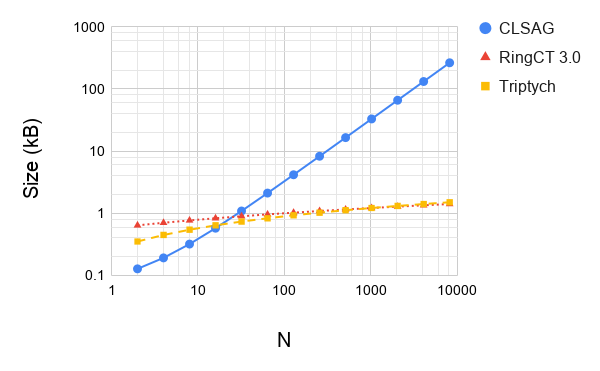
\includegraphics[width=0.6\textwidth]{size.png}
\caption{Total chain growth by anonymity set size}
\label{fig:size}
\end{figure}

\begin{figure}
\centering
\includegraphics[width=0.6\textwidth]{time.png}
\caption{Total verification time by anonymity set size}
\label{fig:time}
\end{figure}

While the updated RingCT 3.0 protocol from \cite{rct3} yields superior space scaling, its requirement that $w$ be a power of two (padded to reach such a value) results in poor verification time scaling.
Comparatively, our construction results in lower overall verification complexity at the expense of overall size scaling.


\bibliographystyle{plain}
\bibliography{main}

\end{document}
